\chapter{Lyhimmät polut}

Lyhimmän polun etsiminen alkusolmusta loppusolmuun
on keskeinen verkko-ongelma, joka esiintyy usein
käytännön tilanteissa.
Esimerkiksi tieverkostossa
tyypillinen ongelma on selvittää,
mikä on lyhin reitti kahden kaupungin välillä,
kun tiedossa ovat kaupunkien väliset tiet ja niiden pituudet.

Jos verkon kaarilla ei ole painoja,
polun pituus on sama kuin kaarten
määrä polulla, jolloin lyhimmän polun
voi etsiä leveyshaulla.
Tässä luvussa keskitymme kuitenkin
tapaukseen, jossa kaarilla on painot.
Tällöin lyhimpien polkujen etsimiseen
tarvitaan kehittyneempiä algoritmeja.

\section{Bellman-Fordin algoritmi}

Bellman-Fordin algoritmi etsii
lyhimmän polun alkusolmusta
kaikkiin muihin verkon solmuihin.
Algoritmi on helppo toteuttaa, ja
sitä voi käyttää kaikenlaisissa verkoissa.
Algoritmi pystyy myös tunnistamaan,
onko verkossa sykliä,
jonka pituus on negatiivinen.

Algoritmi pitää yllä etäisyysarvioita
alkusolmusta kaikkiin muihin verkon solmuihin.
Alussa alkusolmun etäisyysarvio on 0
ja muiden solmujen etäisyys\-arvio on ääretön.
Algoritmi parantaa arvioita
etsimällä verkosta kaaria,
jotka lyhentävät polkuja,
kunnes mitään arviota ei voi enää parantaa.

\subsubsection{Toiminta}

Tarkastellaan Bellman-Fordin
algoritmin toimintaa seuraavassa verkossa:
\begin{center}
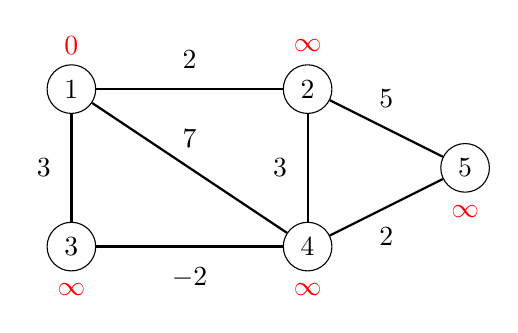
\begin{tikzpicture}
\node[draw, circle] (1) at (1,3) {1};
\node[draw, circle] (2) at (4,3) {2};
\node[draw, circle] (3) at (1,1) {3};
\node[draw, circle] (4) at (4,1) {4};
\node[draw, circle] (5) at (6,2) {5};
\node[color=red] at (1,3+0.55) {$0$};
\node[color=red] at (4,3+0.55) {$\infty$};
\node[color=red] at (1,1-0.55) {$\infty$};
\node[color=red] at (4,1-0.55) {$\infty$};
\node[color=red] at (6,2-0.55) {$\infty$};
\path[draw,thick,-] (1) -- node[font=\small,label=above:2] {} (2);
\path[draw,thick,-] (1) -- node[font=\small,label=left:3] {} (3);
\path[draw,thick,-] (3) -- node[font=\small,label=below:$-2$] {} (4);
\path[draw,thick,-] (2) -- node[font=\small,label=left:3] {} (4);
\path[draw,thick,-] (2) -- node[font=\small,label=above:5] {} (5);
\path[draw,thick,-] (4) -- node[font=\small,label=below:2] {} (5);
\path[draw,thick,-] (1) -- node[font=\small,label=above:7] {} (4);
\end{tikzpicture}
\end{center}
Verkon jokaiseen solmun viereen on merkitty etäisyysarvio.
Alussa alkusolmun etäisyysarvio on 0
ja muiden solmujen etäisyysarvio on
ääretön ($\infty$).

Algoritmin etsii verkosta kaaria,
jotka parantavat etäisyysarvioita.
Aluksi kaikki solmusta 0 lähtevät kaaret
parantavat arvioita:
\begin{center}
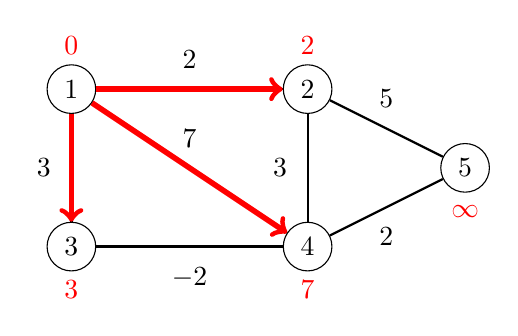
\begin{tikzpicture}
\node[draw, circle] (1) at (1,3) {1};
\node[draw, circle] (2) at (4,3) {2};
\node[draw, circle] (3) at (1,1) {3};
\node[draw, circle] (4) at (4,1) {4};
\node[draw, circle] (5) at (6,2) {5};
\node[color=red] at (1,3+0.55) {$0$};
\node[color=red] at (4,3+0.55) {$2$};
\node[color=red] at (1,1-0.55) {$3$};
\node[color=red] at (4,1-0.55) {$7$};
\node[color=red] at (6,2-0.55) {$\infty$};
\path[draw,thick,-] (1) -- node[font=\small,label=above:2] {} (2);
\path[draw,thick,-] (1) -- node[font=\small,label=left:3] {} (3);
\path[draw,thick,-] (3) -- node[font=\small,label=below:$-2$] {} (4);
\path[draw,thick,-] (2) -- node[font=\small,label=left:3] {} (4);
\path[draw,thick,-] (2) -- node[font=\small,label=above:5] {} (5);
\path[draw,thick,-] (4) -- node[font=\small,label=below:2] {} (5);
\path[draw,thick,-] (1) -- node[font=\small,label=above:7] {} (4);

\path[draw=red,thick,->,line width=2pt] (1) -- (2);
\path[draw=red,thick,->,line width=2pt] (1) -- (3);
\path[draw=red,thick,->,line width=2pt] (1) -- (4);
\end{tikzpicture}
\end{center}

Sitten kaaret $2 \rightarrow 5$ ja $3 \rightarrow 4$
parantavat arvioita:

\begin{center}
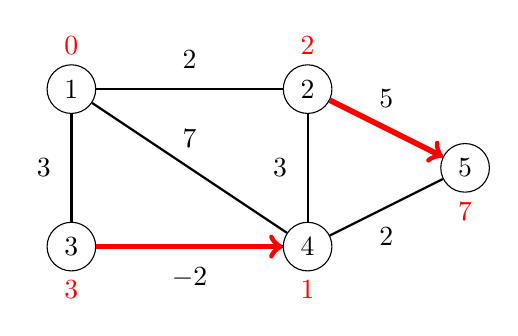
\begin{tikzpicture}
\node[draw, circle] (1) at (1,3) {1};
\node[draw, circle] (2) at (4,3) {2};
\node[draw, circle] (3) at (1,1) {3};
\node[draw, circle] (4) at (4,1) {4};
\node[draw, circle] (5) at (6,2) {5};
\node[color=red] at (1,3+0.55) {$0$};
\node[color=red] at (4,3+0.55) {$2$};
\node[color=red] at (1,1-0.55) {$3$};
\node[color=red] at (4,1-0.55) {$1$};
\node[color=red] at (6,2-0.55) {$7$};
\path[draw,thick,-] (1) -- node[font=\small,label=above:2] {} (2);
\path[draw,thick,-] (1) -- node[font=\small,label=left:3] {} (3);
\path[draw,thick,-] (3) -- node[font=\small,label=below:$-2$] {} (4);
\path[draw,thick,-] (2) -- node[font=\small,label=left:3] {} (4);
\path[draw,thick,-] (2) -- node[font=\small,label=above:5] {} (5);
\path[draw,thick,-] (4) -- node[font=\small,label=below:2] {} (5);
\path[draw,thick,-] (1) -- node[font=\small,label=above:7] {} (4);

\path[draw=red,thick,->,line width=2pt] (2) -- (5);
\path[draw=red,thick,->,line width=2pt] (3) -- (4);
\end{tikzpicture}
\end{center}

Lopuksi tulee vielä yksi parannus:

\begin{center}
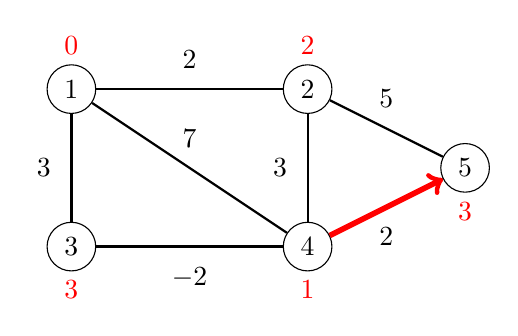
\begin{tikzpicture}
\node[draw, circle] (1) at (1,3) {1};
\node[draw, circle] (2) at (4,3) {2};
\node[draw, circle] (3) at (1,1) {3};
\node[draw, circle] (4) at (4,1) {4};
\node[draw, circle] (5) at (6,2) {5};
\node[color=red] at (1,3+0.55) {$0$};
\node[color=red] at (4,3+0.55) {$2$};
\node[color=red] at (1,1-0.55) {$3$};
\node[color=red] at (4,1-0.55) {$1$};
\node[color=red] at (6,2-0.55) {$3$};
\path[draw,thick,-] (1) -- node[font=\small,label=above:2] {} (2);
\path[draw,thick,-] (1) -- node[font=\small,label=left:3] {} (3);
\path[draw,thick,-] (3) -- node[font=\small,label=below:$-2$] {} (4);
\path[draw,thick,-] (2) -- node[font=\small,label=left:3] {} (4);
\path[draw,thick,-] (2) -- node[font=\small,label=above:5] {} (5);
\path[draw,thick,-] (4) -- node[font=\small,label=below:2] {} (5);
\path[draw,thick,-] (1) -- node[font=\small,label=above:7] {} (4);

\path[draw=red,thick,->,line width=2pt] (4) -- (5);
\end{tikzpicture}
\end{center}

Tämän jälkeen mikään kaari
ei paranna etäisyysarvioita.
Tämä tarkoittaa, että etäisyydet
ovat lopulliset, eli joka solmussa
on nyt pienin etäisyys alkusolmusta
kyseiseen solmuun.

Esimerkiksi pienin etäisyys 3
solmusta 1 solmuun 5 toteutuu käyttämällä
seuraavaa reittiä:

\begin{center}
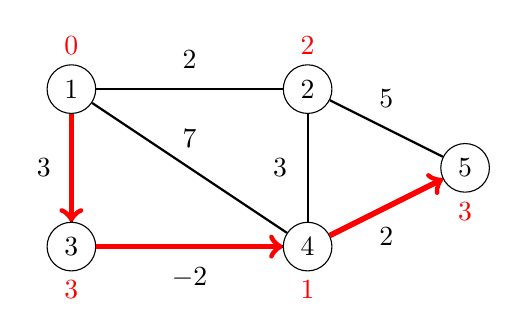
\begin{tikzpicture}
\node[draw, circle] (1) at (1,3) {1};
\node[draw, circle] (2) at (4,3) {2};
\node[draw, circle] (3) at (1,1) {3};
\node[draw, circle] (4) at (4,1) {4};
\node[draw, circle] (5) at (6,2) {5};
\node[color=red] at (1,3+0.55) {$0$};
\node[color=red] at (4,3+0.55) {$2$};
\node[color=red] at (1,1-0.55) {$3$};
\node[color=red] at (4,1-0.55) {$1$};
\node[color=red] at (6,2-0.55) {$3$};
\path[draw,thick,-] (1) -- node[font=\small,label=above:2] {} (2);
\path[draw,thick,-] (1) -- node[font=\small,label=left:3] {} (3);
\path[draw,thick,-] (3) -- node[font=\small,label=below:$-2$] {} (4);
\path[draw,thick,-] (2) -- node[font=\small,label=left:3] {} (4);
\path[draw,thick,-] (2) -- node[font=\small,label=above:5] {} (5);
\path[draw,thick,-] (4) -- node[font=\small,label=below:2] {} (5);
\path[draw,thick,-] (1) -- node[font=\small,label=above:7] {} (4);

\path[draw=red,thick,->,line width=2pt] (1) -- (3);
\path[draw=red,thick,->,line width=2pt] (3) -- (4);
\path[draw=red,thick,->,line width=2pt] (4) -- (5);
\end{tikzpicture}
\end{center}

\subsubsection{Toteutus}

Seuraava Bellman-Fordin algoritmin toteutus
tunnetaan nimellä SPFA-al\-go\-rit\-mi
(\textit{Shortest Path Faster Algorithm}).
Se pitää yllä jonoa solmuista,
joiden kautta kulkevaa polkua saattaa pystyä lyhentämään,
ja valitsee aina seuraavan käsiteltävän solmun
jonon alusta.

Koodi olettaa, että verkko on tallennettuna
vieruslistoina taulukossa \texttt{v}.
Jokainen vieruslista muodostuu pareista,
joissa on ensin kaaren kohdesolmu ja sitten kaaren paino.
Koodi laskee taulukkoon \texttt{e} lyhimmän etäisyyden
alkusolmusta $x$ kaikkiin muihin solmuihin.

Jono \texttt{q} sisältää käsiteltävät verkon solmut:
\begin{lstlisting}
queue<int> q;
\end{lstlisting}

Alussa jonoon lisätään vain solmu $x$.
Koodi käy läpi jonon solmuja ja yrittää lyhentää
polkuja niistä lähtevillä kaarilla.
Aina kun polun pituus lyhenee
kaaren $a \rightarrow b$ ansiosta,
jonoon lisätään solmu $b$.

\begin{lstlisting}
for (int i = 1; i <= n; i++) e[i] = 1e9;
e[x] = 0;
q.push(x);
while (!q.empty()) {
    auto s = q.front(); q.pop();
    for (auto u : v[s]) {
        if (e[s]+u.second < e[u.first]) {
            e[u.first] = e[s]+u.second;
            q.push(u.first);
        }
    }
}
\end{lstlisting}
Algoritmi pysähtyy aina viimeistään $O(nm)$
parannuksen jälkeen, jos verkossa ei ole negatiivista sykliä.
Tämä johtuu siitä, että jokaisessa lyhimmässä polussa
on $O(m)$ kaarta

\subsubsection{Negatiivinen sykli}

Bellman-Fordin algoritmin avulla voi myös tarkastaa,
onko verkossa sykliä,
jonka pituus on negatiivinen.
Esimerkiksi verkossa

\begin{center}
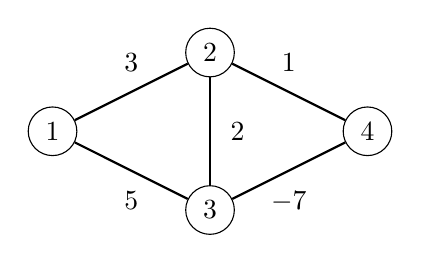
\begin{tikzpicture}
\node[draw, circle] (1) at (0,0) {$1$};
\node[draw, circle] (2) at (2,1) {$2$};
\node[draw, circle] (3) at (2,-1) {$3$};
\node[draw, circle] (4) at (4,0) {$4$};

\path[draw,thick,-] (1) -- node[font=\small,label=above:$3$] {} (2);
\path[draw,thick,-] (2) -- node[font=\small,label=above:$1$] {} (4);
\path[draw,thick,-] (1) -- node[font=\small,label=below:$5$] {} (3);
\path[draw,thick,-] (3) -- node[font=\small,label=below:$-7$] {} (4);
\path[draw,thick,-] (2) -- node[font=\small,label=right:$2$] {} (3);
\end{tikzpicture}
\end{center}
\noindent
on negatiivinen sykli $2 \rightarrow 3 \rightarrow 4 \rightarrow 2$,
jonka pituus on $-4$.

Jos verkossa on negatiivinen sykli,
sen kautta kulkevaa polkua voi lyhentää äärettömästi
toistamalla negatiivista sykliä uudestaan ja uudestaan,
minkä vuoksi lyhimmän polun käsite ei ole mielekäs.

Negatiivisen syklin voi tunnistaa
Bellman-Fordin algoritmilla
alustamalla ensin kaikki etäisyysarviot nolliksi
ja suorittamalla sitten
algoritmia $n$ kierrosta.
Jos viimeinen kierros parantaa jotain
etäisyysarviota, verkossa on negatiivinen sykli.
Huomaa, että tässä mikään solmuista ei ole alkusolmu
ja algoritmi etsii negatiivista sykliä koko verkon alueelta.

\section{Dijkstran algoritmi}

Dijkstran algoritmi etsii Bellman-Fordin
algoritmin tavoin lyhimmät polut
alkusolmusta kaikkiin muihin solmuihin.
Dijkstran algoritmi on tehokkaampi kuin
Bellman-Fordin algoritmi,
minkä ansiosta se soveltuu suurten
verkkojen käsittelyyn.
Algoritmi vaatii kuitenkin,
ettei verkossa ole negatiivisia kaaria.

Dijkstran algoritmi vastaa
Bellman-Fordin algoritmia siinä,
että se pitää
yllä etäisyysarvioita solmuihin
ja parantaa niitä algoritmin aikana.
Algoritmin tehokkuus perustuu
siihen, että sen riittää käydä läpi
verkon kaaret vain kerran
hyödyntäen tietoa,
ettei verkossa ole negatiivisia kaaria.

\subsubsection{Toiminta}

Tarkastellaan Dijkstran algoritmin toimintaa
seuraavassa verkossa:
\begin{center}
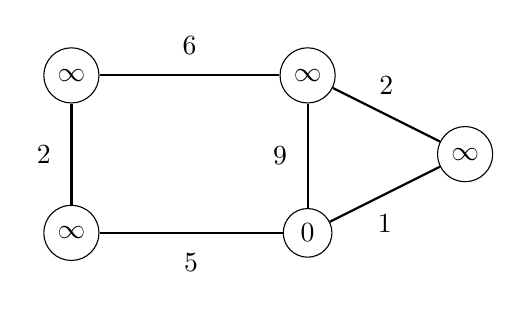
\begin{tikzpicture}
\node[draw, circle] (1) at (1,3) {$\infty$};
\node[draw, circle] (2) at (4,3) {$\infty$};
\node[draw, circle] (3) at (1,1) {$\infty$};
\node[draw, circle] (4) at (4,1) {$0$};
\node[draw, circle] (5) at (6,2) {$\infty$};

\path[draw,thick,-] (1) -- node[font=\small,label=above:6] {} (2);
\path[draw,thick,-] (1) -- node[font=\small,label=left:2] {} (3);
\path[draw,thick,-] (3) -- node[font=\small,label=below:5] {} (4);
\path[draw,thick,-] (2) -- node[font=\small,label=left:9] {} (4);
\path[draw,thick,-] (2) -- node[font=\small,label=above:2] {} (5);
\path[draw,thick,-] (4) -- node[font=\small,label=below:1] {} (5);
\end{tikzpicture}
\end{center}
Bellman-Fordin algoritmin tavoin
alkusolmun etäisyysarvio on 0
ja kaikissa muissa solmuissa etäisyysarvio
on aluksi $\infty$.

Dijkstran algoritmi
ottaa joka askeleella käsittelyyn
sellaisen solmun,
jota ei ole vielä käsitelty
ja jonka etäisyysarvio on
mahdollisimman pieni.
Alussa tällainen solmu on alkusolmu,
jonka etäisyysarvio on 0.

Kun solmu tulee käsittelyyn,
algoritmi käy läpi kaikki
siitä lähtevät kaaret ja
parantaa etäisyysarvioita
niiden avulla:
\begin{center}
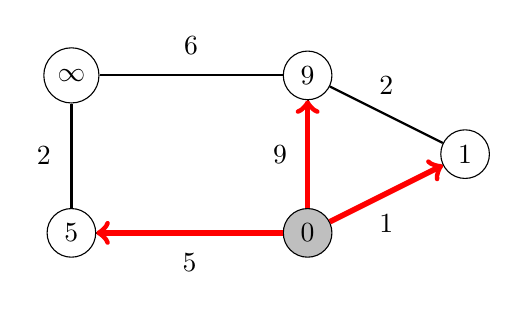
\begin{tikzpicture}
\node[draw, circle] (1) at (1,3) {$\infty$};
\node[draw, circle] (2) at (4,3) {$9$};
\node[draw, circle] (3) at (1,1) {$5$};
\node[draw, circle, fill=lightgray] (4) at (4,1) {$0$};
\node[draw, circle] (5) at (6,2) {$1$};

\path[draw,thick,-] (1) -- node[font=\small,label=above:6] {} (2);
\path[draw,thick,-] (1) -- node[font=\small,label=left:2] {} (3);
\path[draw,thick,-] (3) -- node[font=\small,label=below:5] {} (4);
\path[draw,thick,-] (2) -- node[font=\small,label=left:9] {} (4);
\path[draw,thick,-] (2) -- node[font=\small,label=above:2] {} (5);
\path[draw,thick,-] (4) -- node[font=\small,label=below:1] {} (5);

\path[draw=red,thick,->,line width=2pt] (4) -- (2);
\path[draw=red,thick,->,line width=2pt] (4) -- (3);
\path[draw=red,thick,->,line width=2pt] (4) -- (5);
\end{tikzpicture}
\end{center}
Alkusolmun käsittely paransi etäisyysarvioita
kolmen muuhun solmuun,
joiden uudet etäisyydet ovat nyt 1, 5 ja 9.

\begin{samepage}
Seuraavaksi käsittelyyn tulee solmu,
jonka etäisyys on 1:

\begin{center}
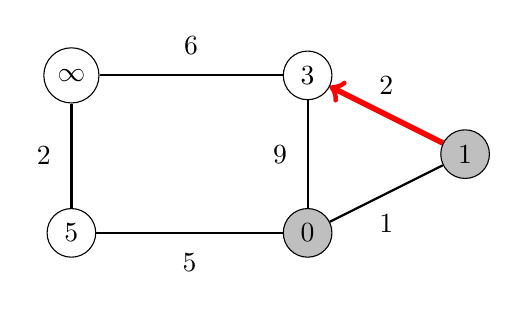
\begin{tikzpicture}
\node[draw, circle] (1) at (1,3) {$\infty$};
\node[draw, circle] (2) at (4,3) {$3$};
\node[draw, circle] (3) at (1,1) {$5$};
\node[draw, circle, fill=lightgray] (4) at (4,1) {$0$};
\node[draw, circle, fill=lightgray] (5) at (6,2) {$1$};

\path[draw,thick,-] (1) -- node[font=\small,label=above:6] {} (2);
\path[draw,thick,-] (1) -- node[font=\small,label=left:2] {} (3);
\path[draw,thick,-] (3) -- node[font=\small,label=below:5] {} (4);
\path[draw,thick,-] (2) -- node[font=\small,label=left:9] {} (4);
\path[draw,thick,-] (2) -- node[font=\small,label=above:2] {} (5);
\path[draw,thick,-] (4) -- node[font=\small,label=below:1] {} (5);

\path[draw=red,thick,->,line width=2pt] (5) -- (2);
\end{tikzpicture}
\end{center}
\end{samepage}

Tämän jälkeen vuorossa on solmu 3:

\begin{center}
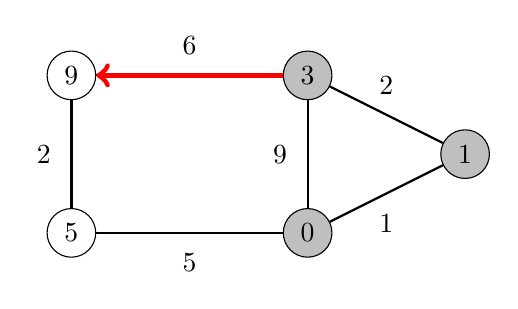
\begin{tikzpicture}
\node[draw, circle] (1) at (1,3) {$9$};
\node[draw, circle, fill=lightgray] (2) at (4,3) {$3$};
\node[draw, circle] (3) at (1,1) {$5$};
\node[draw, circle, fill=lightgray] (4) at (4,1) {$0$};
\node[draw, circle, fill=lightgray] (5) at (6,2) {$1$};

\path[draw,thick,-] (1) -- node[font=\small,label=above:6] {} (2);
\path[draw,thick,-] (1) -- node[font=\small,label=left:2] {} (3);
\path[draw,thick,-] (3) -- node[font=\small,label=below:5] {} (4);
\path[draw,thick,-] (2) -- node[font=\small,label=left:9] {} (4);
\path[draw,thick,-] (2) -- node[font=\small,label=above:2] {} (5);
\path[draw,thick,-] (4) -- node[font=\small,label=below:1] {} (5);

\path[draw=red,thick,->,line width=2pt] (2) -- (1);
\end{tikzpicture}
\end{center}

Dijkstran algoritmissa on hienoutena,
että aina kun solmu tulee käsittelyyn,
sen etäisyysarvio on siitä lähtien lopullinen.
Esimerkiksi tässä vaiheessa
etäisyydet 0, 1 ja 3 ovat lopulliset
etäisyydet käsiteltyihin solmuihin.

Algoritmi käsittelee vastaavasti
vielä kaksi viimeistä solmua,
minkä jälkeen algoritmin päätteeksi
etäisyydet ovat:

\begin{center}
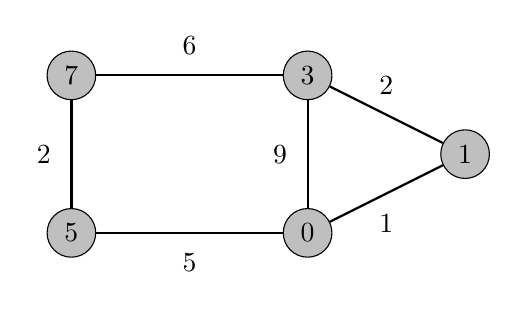
\begin{tikzpicture}
\node[draw, circle, fill=lightgray] (1) at (1,3) {$7$};
\node[draw, circle, fill=lightgray] (2) at (4,3) {$3$};
\node[draw, circle, fill=lightgray] (3) at (1,1) {$5$};
\node[draw, circle, fill=lightgray] (4) at (4,1) {$0$};
\node[draw, circle, fill=lightgray] (5) at (6,2) {$1$};

\path[draw,thick,-] (1) -- node[font=\small,label=above:6] {} (2);
\path[draw,thick,-] (1) -- node[font=\small,label=left:2] {} (3);
\path[draw,thick,-] (3) -- node[font=\small,label=below:5] {} (4);
\path[draw,thick,-] (2) -- node[font=\small,label=left:9] {} (4);
\path[draw,thick,-] (2) -- node[font=\small,label=above:2] {} (5);
\path[draw,thick,-] (4) -- node[font=\small,label=below:1] {} (5);
\end{tikzpicture}
\end{center}

\subsubsection{Negatiiviset kaaret}

Dijkstran algoritmin tehokkuus perustuu siihen,
että verkossa ei ole negatiivisia kaaria.
Jos verkossa on negatiivinen kaari,
algoritmi ei välttämättä toimi oikein.
Esimerkiksi verkossa

\begin{center}
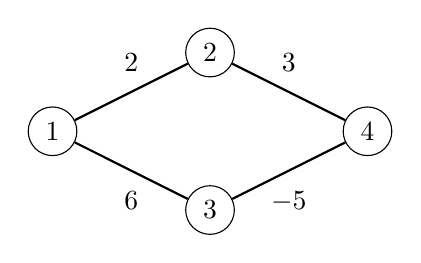
\begin{tikzpicture}
\node[draw, circle] (1) at (0,0) {$1$};
\node[draw, circle] (2) at (2,1) {$2$};
\node[draw, circle] (3) at (2,-1) {$3$};
\node[draw, circle] (4) at (4,0) {$4$};

\path[draw,thick,-] (1) -- node[font=\small,label=above:2] {} (2);
\path[draw,thick,-] (2) -- node[font=\small,label=above:3] {} (4);
\path[draw,thick,-] (1) -- node[font=\small,label=below:6] {} (3);
\path[draw,thick,-] (3) -- node[font=\small,label=below:$-5$] {} (4);
\end{tikzpicture}
\end{center}
\noindent
solmusta 1 alkaen Dijkstran algoritmi löytää keveimpiä kaaria seuraamalla
reitin $1 \rightarrow 2 \rightarrow 4$,
vaikka lyhyempi reitti olisi $1 \rightarrow 3 \rightarrow 4$.

\subsubsection{Toteutus}

Seuraava Dijkstran algoritmin toteutus laskee
pienimmän etäisyyden solmusta $s$ kaikkiin muihin solmuihin.
Verkossa on $n$ solmua ja $m$ kaarta,
ja tiedot kaarista on tallennettu taulukkoon \texttt{v}
vieruslistoina, joissa on pareina kohdesolmu
ja kaaren pituus.

Dijkstran algoritmin tehokas toteutus vaatii,
että verkosta on mahdollista
löytää nopeasti vielä käsittelemätön solmu,
jonka etäisyysarvio on pienin.
Sopiva tietorakenne tähän on prioriteettijono,
jossa solmut ovat järjestyksessä etäisyysarvioiden mukaan.
Prioriteettijonon avulla
seuraavaksi käsiteltävän solmun saa selville logaritmisessa ajassa.

Seuraavassa toteutuksessa prioriteettijono sisältää
pareja, joiden ensimmäinen kenttä on etäisyysarvio
ja toinen kenttä on solmun tunniste:
\begin{lstlisting}
priority_queue<pair<int,int>> q;
\end{lstlisting}
Pieni hankaluus on,
että Dijkstran algoritmissa täytyy saada selville
pienimmän etäisyysarvion solmu,
kun taas C++:n prioriteettijono antaa oletuksena
suurimman alkion.
Helppo ratkaisu on tallentaa etäisyysarviot
\textit{negatiivisina}, jolloin C++:n prioriteettijonoa
voi käyttää suoraan.

Koodi käyttää lisäksi taulukoita
\texttt{z} ja \texttt{e},
joissa on alkio jokaiselle solmulle $i$
välillä $1 \le i \le n$.
Taulukko $\texttt{z}$ kertoo,
onko solmu jo käsitely,
ja sen jokainen alkio on 0 (ei käsitelty)
tai 1 (käsitelty).
Taulukossa \texttt{e} taas on etäisyysarviot
solmusta $s$ kaikkiin solmuihin.
Alussa alkusolmun etäisyysarvio on 0
ja jokaisen muun solmun etäisyysarviona
on ääretöntä vastaava $10^9$.

\begin{lstlisting}
for (int i = 1; i <= n; i++) e[i] = 1e9;
e[s] = 0;
q.push({0,s});
while (!q.empty()) {
    int x = q.top().second;
    q.pop();
    if (z[x]) continue;
    z[x] = 1;
    for (int i = 0; i < v[x].size(); i++) {
        int u = v[x][i].first;
        if (e[x]+v[x][i].second < e[u]) {
            e[u] = e[x]+v[x][i].second;
            q.push({-e[u],u});
        }
    }
}
\end{lstlisting}

Yllä olevan toteutuksen aikavaativuus on $O(n+m \log m)$,
koska algoritmi käy läpi kaikki verkon solmut
ja lisää jokaista kaarta kohden korkeintaan
yhden etäisyysarvion prioriteettijonoon.
Jokainen prioriteettijonon operaatio vie aikaa
$O(\log m)$ ja operaatioita tehdään kaikkiaan
$O(m)$ kappaletta,
joten prioriteettijonon käsittelyyn
kuluu aikaa yhteensä $O(m \log m)$.

\section{Floyd-Warshallin algoritmi}

Floyd-Warshallin algoritmi on toisenlainen
lähestymistapa lyhimpien polkujen
etsimiseen kuin Bellman-Fordin ja
Dijkstran algoritmit.
Siinä missä muut algoritmit
etsivät lyhimpiä polkuja
tietystä solmusta alkaen,
Floyd-Warshallin algoritmi etsii
lyhimmän polun jokaisen verkon
solmuparin välillä.

Algoritmi ylläpitää kaksiulotteista
taulukkoa etäisyyksistä solmujen
välillä.
Ensin taulukkoon on merkitty
etäisyydet käyttäen vain solmujen
välisiä kaaria.
Tämän jälkeen algoritmi
päivittää etäisyyksiä,
kun verkon solmut saavat yksi kerrallaan
toimia välisolmuina poluilla.

\subsubsection{Toiminta}

Tarkastellaan Floyd-Warshallin
algoritmin toimintaa seuraavassa verkossa:

\begin{center}
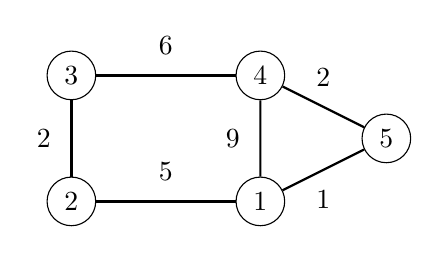
\begin{tikzpicture}[scale=0.80]
\node[draw, circle] (1) at (1,3) {$3$};
\node[draw, circle] (2) at (4,3) {$4$};
\node[draw, circle] (3) at (1,1) {$2$};
\node[draw, circle] (4) at (4,1) {$1$};
\node[draw, circle] (5) at (6,2) {$5$};

\path[draw,thick,-] (1) -- node[font=\small,label=above:6] {} (2);
\path[draw,thick,-] (1) -- node[font=\small,label=left:2] {} (3);
\path[draw,thick,-] (3) -- node[font=\small,label=above:5] {} (4);
\path[draw,thick,-] (2) -- node[font=\small,label=left:9] {} (4);
\path[draw,thick,-] (2) -- node[font=\small,label=above:2] {} (5);
\path[draw,thick,-] (4) -- node[font=\small,label=below:1] {} (5);
\end{tikzpicture}
\end{center}

Algoritmi merkitsee aluksi taulukkoon
etäisyyden 0 jokaisesta solmusta itseensä
sekä etäisyyden $x$, jos solmuparin välillä
on kaari, jonka pituus on $x$.
Muiden solmuparien etäisyys on aluksi ääretön.

Tässä verkossa taulukosta tulee:
\begin{center}
\begin{tabular}{r|rrrrr}
 & 1 & 2 & 3 & 4 & 5 \\
\hline
1 & 0 & 5 & $\infty$ & 9 & 1 \\
2 & 5 & 0 & 2 & $\infty$ & $\infty$ \\
3 & $\infty$ & 2 & 0 & 6 & $\infty$ \\
4 & 9 & $\infty$ & 6 & 0 & 2 \\
5 & 1 & $\infty$ & $\infty$ & 2 & 0 \\
\end{tabular}
\end{center}
\vspace{10pt}
Algoritmin toiminta muodostuu peräkkäisistä kierroksista.
Jokaisella kierroksella uusi solmu saa
toimia välisolmuna poluilla,
ja algoritmi parantaa taulukon
etäisyyksiä muodostaen polkuja tämän solmun avulla.

Ensimmäisellä kierroksella solmu 1 on välisolmu.
Tämän ansiosta solmujen 2 ja 4 välille muodostuu
polku, jonka pituus on 14,
koska solmu 1 yhdistää ne toisiinsa.
Vastaavasti solmut 2 ja 5 yhdistyvät polulla,
jonka pituus on 6.

\begin{center}
\begin{tabular}{r|rrrrr}
 & 1 & 2 & 3 & 4 & 5 \\
\hline
1 & 0 & 5 & $\infty$ & 9 & 1 \\
2 & 5 & 0 & 2 & \textbf{14} & \textbf{6} \\
3 & $\infty$ & 2 & 0 & 6 & $\infty$ \\
4 & 9 & \textbf{14} & 6 & 0 & 2 \\
5 & 1 & \textbf{6} & $\infty$ & 2 & 0 \\
\end{tabular}
\end{center}
\vspace{10pt}

Toisella kierroksella myös solmu 2 saa toimia välisolmuna.
Tämä mahdollistaa uudet polut solmuparien 1 ja 3
sekä 3 ja 5 välille:

\begin{center}
\begin{tabular}{r|rrrrr}
 & 1 & 2 & 3 & 4 & 5 \\
\hline
1 & 0 & 5 & \textbf{7} & 9 & 1 \\
2 & 5 & 0 & 2 & 14 & 6 \\
3 & \textbf{7} & 2 & 0 & 6 & \textbf{8} \\
4 & 9 & 14 & 6 & 0 & 2 \\
5 & 1 & 6 & \textbf{8} & 2 & 0 \\
\end{tabular}
\end{center}
\vspace{10pt}

Algoritmin toiminta jatkuu samalla tavalla
niin, että kukin solmu tulee vuorollaan
välisolmuksi.
Algoritmin päätteeksi taulukko sisältää
lyhimmän etäisyyden minkä tahansa
solmuparin välillä:

\begin{center}
\begin{tabular}{r|rrrrr}
 & 1 & 2 & 3 & 4 & 5 \\
\hline
1 & 0 & 5 & 7 & 3 & 1 \\
2 & 5 & 0 & 2 & 8 & 6 \\
3 & 7 & 2 & 0 & 6 & 8 \\
4 & 3 & 8 & 6 & 0 & 2 \\
5 & 1 & 6 & 8 & 2 & 0 \\
\end{tabular}
\end{center}

\subsubsection{Toteutus}

Floyd-Warshallin algoritmin etuna on,
että se on helppoa toteuttaa.
Seuraava toteutus muodostaa etäisyysmatriisin
\texttt{d}, jossa $\texttt{d}[a][b]$
on pienin etäisyys polulla solmusta $a$ solmuun $b$.
Alussa $\texttt{d}[a][b]=0$, jos $a=b$,
$\texttt{d}[a][b]=x$, jos $a$:sta $b$:hen
on $x$-pituinen kaari,
ja muuten $\texttt{d}[a][b]=\infty$.

Tämän jälkeen lyhimmät polut löytyvät seuraavasti:

\begin{lstlisting}
for (int k = 1; k <= n; k++) {
    for (int i = 1; i <= n; i++) {
        for (int j = 1; j <= n; j++) {
            d[i][j] = min(d[i][j], d[i][k]+d[k][j]);
        }
    }
}
\end{lstlisting}

Algoritmin aikavaativuus on
$O(n^3)$, koska siinä on kolme sisäkkäistä
silmukkaa,
jotka käyvät läpi verkon solmut.

Koska algoritmin toteutus on yksinkertainen,
se voi olla hyvä valinta jopa silloin,
kun haettavana on yksittäinen
lyhin polku verkossa.
Tämä vaatii kuitenkin, että verkko on pieni
ja kuutiollinen aikavaativuus on riittävä.

